\documentclass[ ]{article}
\title{Revisão P2 \\ Divane Marcon}
\author{Erickson G. Müller}
\date{25 de Junho de 2024}

\usepackage[ ]{tikz}
\usepackage[ ]{pgfplots}
\usepackage[ ]{amsmath}
\usepackage[ ]{graphicx}

\begin{document}
\maketitle

\section{Conteúdos}
	\begin{enumerate}
		\item Derivadas
		\item Velocidade e Aceleração
		\item Integrais Definidas e Indefinidas
		\item Teorema Fundamental do Cálculo
		\item Cálculo de Áreas
	\end{enumerate}
\newpage

\section{Derivadas}
	A derivada é o coeficiente angular da reta tangente à curva f(x) num determinado ponto.\\
	
	\begin{minipage}{6 cm}
		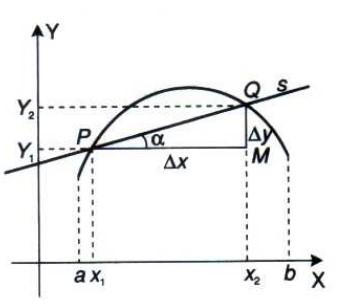
\includegraphics[scale=0.58]{Images/Graph1.jpg}
	\end{minipage}		
	\begin{minipage}{6 cm}
		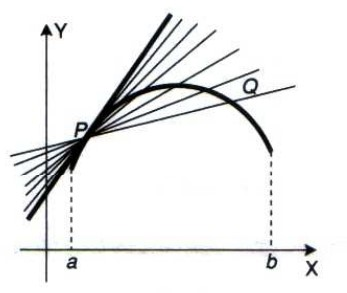
\includegraphics[scale=0.6]{Images/Graph2.jpg}
	\end{minipage}
	
	A curva tangente no ponto P	é calculada à medida que o ponto Q se aproxima do ponto P correndo sobre a curva.
	$$\lim_{Q_x\to P_x}f(x)=P'x+b$$
	Exemplo:\\
	Encontre a inclinação da reta tangente à curva $y=x^2-2x+1$ no ponto $(x_1,y_1)$.\\
	
	Se $f(x)=x^2-2x+1$, então $f(x)=x_1^2-2x_1+1$;\\
	$$f(x_1+\Delta x)=(x_1+\Delta x)^2 -2.(x_1+\Delta x) + 1$$
	$$=x_1^2+2.x_1.\Delta x + \Delta x^2 - 2.x_1 -2.\Delta x +1$$
	
	Usando limites...
	
	$$m(x_1) = \lim_{\Delta x \to 0}\dfrac{f(x_1+\Delta x)-f(x_1)}{\Delta x}$$
	$$=\lim_{\Delta x\to 0}\dfrac{x_1^2+2.x_1.\Delta x + \Delta x^2 - 2.x_1 -2.\Delta x +1 - (x_1^2-2x_1+1)}{\Delta x}$$
	$$=\lim_{\Delta x\to 0}\dfrac{2.x_1.\Delta x + \Delta x^2-2\Delta x}{\Delta x}$$
	$$ = \lim_{\Delta x\to 0}\dfrac{\Delta x.(2.x_1+\Delta x -2)}{\Delta x} = 2.x_1 - 2$$
	
	Por meio dessa derivação, provamos a propriedade de que $f'(x) = n.x^{n-1}$.
	\newpage
	Para entender melhor, irei desenhar um gráfico com as curvas $x^2-2x+1$ e $(2x-2).x+b$, para $x=3$:\\
	Ou seja, o $2x+b$ passa a ser o a da nova reta a ser descoberta, deste modo, se quisermos que a reta passe no ponto $(3,4)$, aplicaremos na fórmula da reta $y = ax+b$.
	$$4 = (2.3-2).3 + b$$
	$$a = 4$$ $$b=-8$$
	$$f'(x) = 4x - 8$$
	
	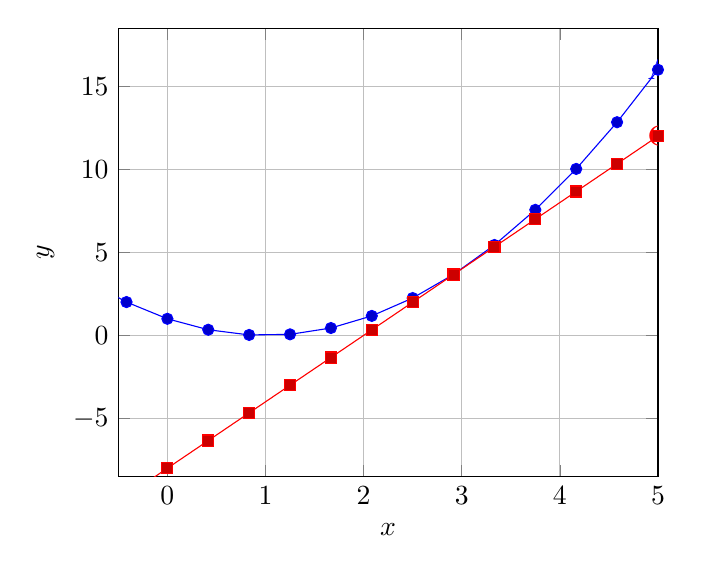
\begin{tikzpicture}
		\begin{axis}[
    		xlabel={$x$},
		    ylabel={$y$},
		    xmin = -0.5,  % Replace with your xmin value
		    xmax = 5,  % Replace with your xmax value
		    ymin = -8.5,  % This will be automatically calculated
		    ymax = 18.5,  % This will be automatically calculated
		    grid = major,]
		    
		    \addplot {x^2-2*x+1} node {A};
		    %\addplot {2*x-2} node {B};
		    \addplot {(2*3-2)*x - (2*3-2)*2} node {C};
		\end{axis}
	\end{tikzpicture}
	
	\subsection{Propriedades}
		\begin{enumerate}
			\item Embora exista limite em ponto anguloso, não existe derivada nesse ponto pois o coeficiente angular à esquerda e à direita são diferentes.
			\item Se $f(x) = x^n$, então $f'(x) = n.x^{n-1}$
				
			\item A derivada de uma constante é 0.
			
			\item A derivada do produto de uma constante por um função é essa derivada multiplicada pela constante. $g(x) = k.f(x)$ logo $g'(x) = k.f'(x)$		
			
			\item A derivada da soma de duas funções é a soma das derivadas das duas funções. $h(x) = f(x) + g(x)$ logo $h'(x) = f'(x) + g'(x)$
		\end{enumerate}
	\subsection{Derivada de uma Função num Ponto}
		A derivada da função $f(x)$ no ponto $x_1$, denotada por $f'(x_1)$, é definida pelo limite:
		
		$$f'(x) = \lim_{\Delta x\to 0} \dfrac{f(x_1+\Delta x)-f(x_1)}{\Delta x}$$
		ou
		$$f'(x) = \lim_{x_f\to x_0}\dfrac{f(x_f)-f(x_0)}{x_f-x_0}$$	
		
	\subsection{Velocidade e Aceleração}
		Existem dois tipos de cálculo para encontrar uma velocidade ou aceleração, a velocidade ou aceleração instantâneas e a velocidade e aceleração intervalares. A intervalar é calculada fazendo a média da diferença entre as distâncias ou as velocidades em um determinado intervalo de tempo ($\frac{s(t+\Delta t)-s(t)}{\Delta t}$). Para calcularmos a velocidade em determinado momento, precisamos aplicar o limite das velocidades médias quando $\Delta t$ se aproxima de 0.
		
		$$v(\Delta t) = \frac{s(t+\Delta t)-s(t)}{\Delta t}$$
		$$v(t) =\lim_{\Delta t\to 0}\frac{s(t+\Delta t)-s(t)}{\Delta t}= s'(t)$$
		
		Para calcular a aceleração, em vez da velocidade, apenas se substituem na fórmula as variáveis distância(s) pelas variáveis velocidade(v). Assim como a velocidade é calculada pela variação de distância, a aceleração é calculada pela variação de velocidade.
		
	\subsection{Regra da Cadeia}
	\subsection{Derivada das Funções Elementares}
		
	\subsection{Derivada das Funções Trigonométricas}
	
\newpage
\section{Exemplos Derivada no Ponto}
	\subsection{Reta Tangente que seja Paralela a Outra Reta}	
		Encontre a equação da reta tangente à curva $y = \sqrt{x}$ que seja paralela à reta $8.x - 4.y + 1 = 0$.\\
		Por serem paralelas, seus coeficientes angulares são iguais.\\
		Por esse motivo vamos encontrar a inclinação da reta tangente à curva $y = \sqrt{x}$ num ponto $(x_1,y_1)$. Temos:
		$$f'(x) = \lim_{\Delta x\to 0}\dfrac{\sqrt[]{x_1 + \Delta x}-\sqrt[ ]{x_1}}{\Delta x}$$

		$$= \lim_{\Delta x\to 0}\dfrac{\sqrt[]{x_1 + \Delta x}-\sqrt[ ]{x_1}}{\Delta x}.\dfrac{(\sqrt[ ]{x_1+\Delta x}+\sqrt[ ]{x_1})}{(\sqrt[ ]{x_1+\Delta x}+\sqrt[ ]{x_1})}$$

		$$= \lim_{\Delta x \to 0}\dfrac{\sqrt[ ]{x_1+\Delta x}^2-\sqrt[ ]{x_1}^2}  {\Delta x.(\sqrt[ ]{x_1 + \Delta x}+ \sqrt[ ]{x_1})}$$		
		
		$$= \lim_{\Delta x \to 0}\dfrac{x_1+\Delta x-x_1}{\Delta x.(\sqrt[ ]{x_1 + \Delta x}+ \sqrt[ ]{x_1})}$$
		
		$$f'(x) = \lim_{\Delta x\to 0}\dfrac{1}{\sqrt[ ]{x_1+\Delta x}+ \sqrt[ ]{x_1}}$$
		$$f'(x) = \dfrac{1}{2.\sqrt[ ]{x_1}}$$
		
		Essa é a derivada de $f(x) = \sqrt[ ]{x}$, como queremos encontrar a reta tangente que seja paralela à reta $8.x-4.y+1=0$, precisamos igualar a derivada de $f(x)$ ao coeficiente angular da segunda reta. \textbf{Pois a derivada de uma curva é o coeficiente angular da reta tangente à curva em determinado ponto.}
		
		$$\dfrac{1}{2.\sqrt[ ]{x_1}}=\dfrac{8}{4}$$
		$$\sqrt[ ]{x_1}=\dfrac{1}{4}$$
		$$x_1 = \dfrac{1}{16}$$
		$$y_1 = \dfrac{1}{4}$$

		Esse é o ponto da reta tangente. Podemos agora aplicar à fórmula da função de segundo grau:

		$$\dfrac{1}{4}=2.\dfrac{1}{16}+b$$
		$$b =\dfrac{2}{8}-\dfrac{1}{8}=\dfrac{1}{8}$$
		$$y=2.x+\dfrac{1}{8}$$
		$$16.x-8.y+1=0$$
		
	\subsection{Reta Tangente que seja Perpendicular a Outra Reta}
		No último exemplo, encontramos a derivada usando uma reta paralela à reta a qual buscamos, para isso a derivada da função deve ser igual ao coeficiente angular da reta paralela. Agora vamos ver um exemplo de como encontrar uma reta tangente que seja perpendicular a uma outra reta.\\
		\textbf{O nome dessa reta perpendicular é reta normal} e ela apresenta ângulo reto no ponto da reta tangente.\\
		\includegraphics[scale=0.3]{Images/reta normal.png}
		\\
		Acima temos a equação para a reta normal à curva $y = x²$ no ponto $(2,4)$.\\
		Duas retas $f(x)$ e $g(x)$ são perpendiculares se o \textbf{produto dos coeficientes angulares das duas retas for igual a -1}.

	\subsection{Derivada Conforme Valor de x}
	Dada $f(x)=\sqrt[]{x}$, encontre $f'(4)$.

	$$f'(x)=\lim_{x\to x_1}\dfrac{f(x)-f(x_1)}{x-x_1}$$	

	Em vez de aproximarmos o $\Delta x$ a $0$, aproximamos o $x$ ao valor de $x$ para aquele ponto.

	$$f'(x) = \lim_{x\to 4}\dfrac{\sqrt[ ]{x}-\sqrt[•]{4}}{x-4}$$
	
	$$= \lim_{x\to 4}\dfrac{\sqrt[•]{x}-2}{x-4}.\dfrac{\sqrt[]{x}+2}{\sqrt[•]{x}+2}$$
	\textit{Quando os números do denominador forem o quadrado destes no numerador, multiplicar pela soma/subtração destes mesmos, conforme a operação no numerador.}
	
	$$= \lim_{x\to 4}\dfrac{x-4}{(x-4).(\sqrt[•]{x}+2)}$$
	
	$$= \lim_{x\to 4}\dfrac{1}{\sqrt[•]{x}+2} = \dfrac{1}{4}$$
	
	
\newpage
\section{Integrais}
	\subsection{Integrais Definidas}
	\subsection{Integrais Indefinidas}
	\subsection{Teorema Fundamental do Cálculo}
\section{Cálculo de Áreas}
	
\end{document}